\chapter{Выполнение задания}

\section{Реализуемый алгоритм}
Сортировка слиянием

\section{Выбор языка программирования}
Для выполнения домашнего задания был выбран язык \texttt{C++}.

\section{Код программы}

В листинге \ref{lst:merge} приведена реализация алгоритма сортировки слиянием.

\lstinputlisting[label=lst:merge, caption=Реализация алгоритма сортировки слиянием, firstline=13,lastline=55]{../code/main.cpp}

\section{Модели программ}

На рисунках \ref{fg:mg}--\ref{fg:ii} представлены модели графовых управлений.

\subsection{Граф управления программы}

\begin{figure}[h]
	\centering
	\label{fg:mg}
	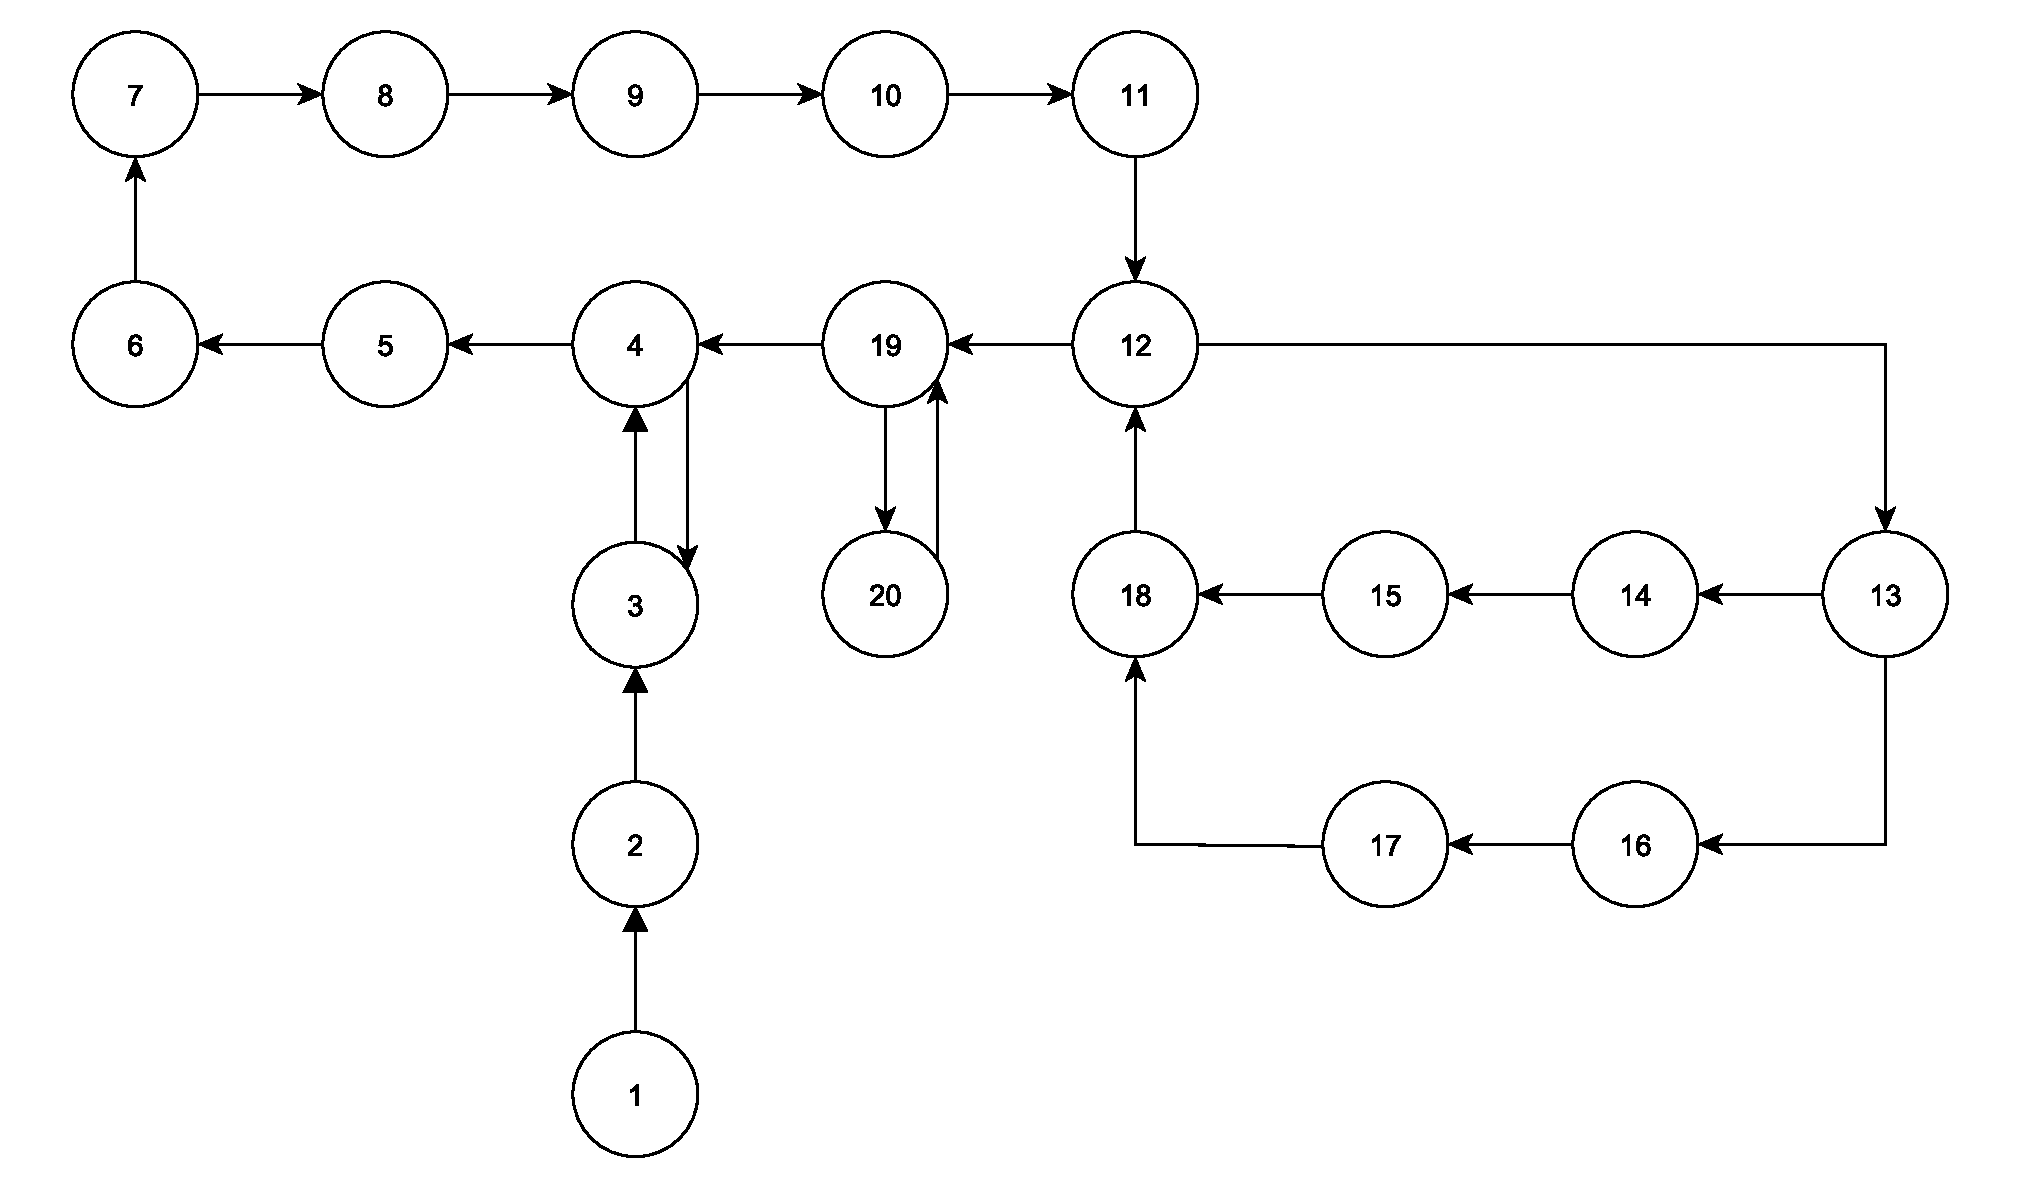
\includegraphics[height=0.2\textheight]{img/граф_управления.pdf}
	\caption{Граф управления}
\end{figure}

\clearpage

\subsection{Информационный граф программы}

\begin{figure}[h]
	\centering
	\label{fg:ig}
	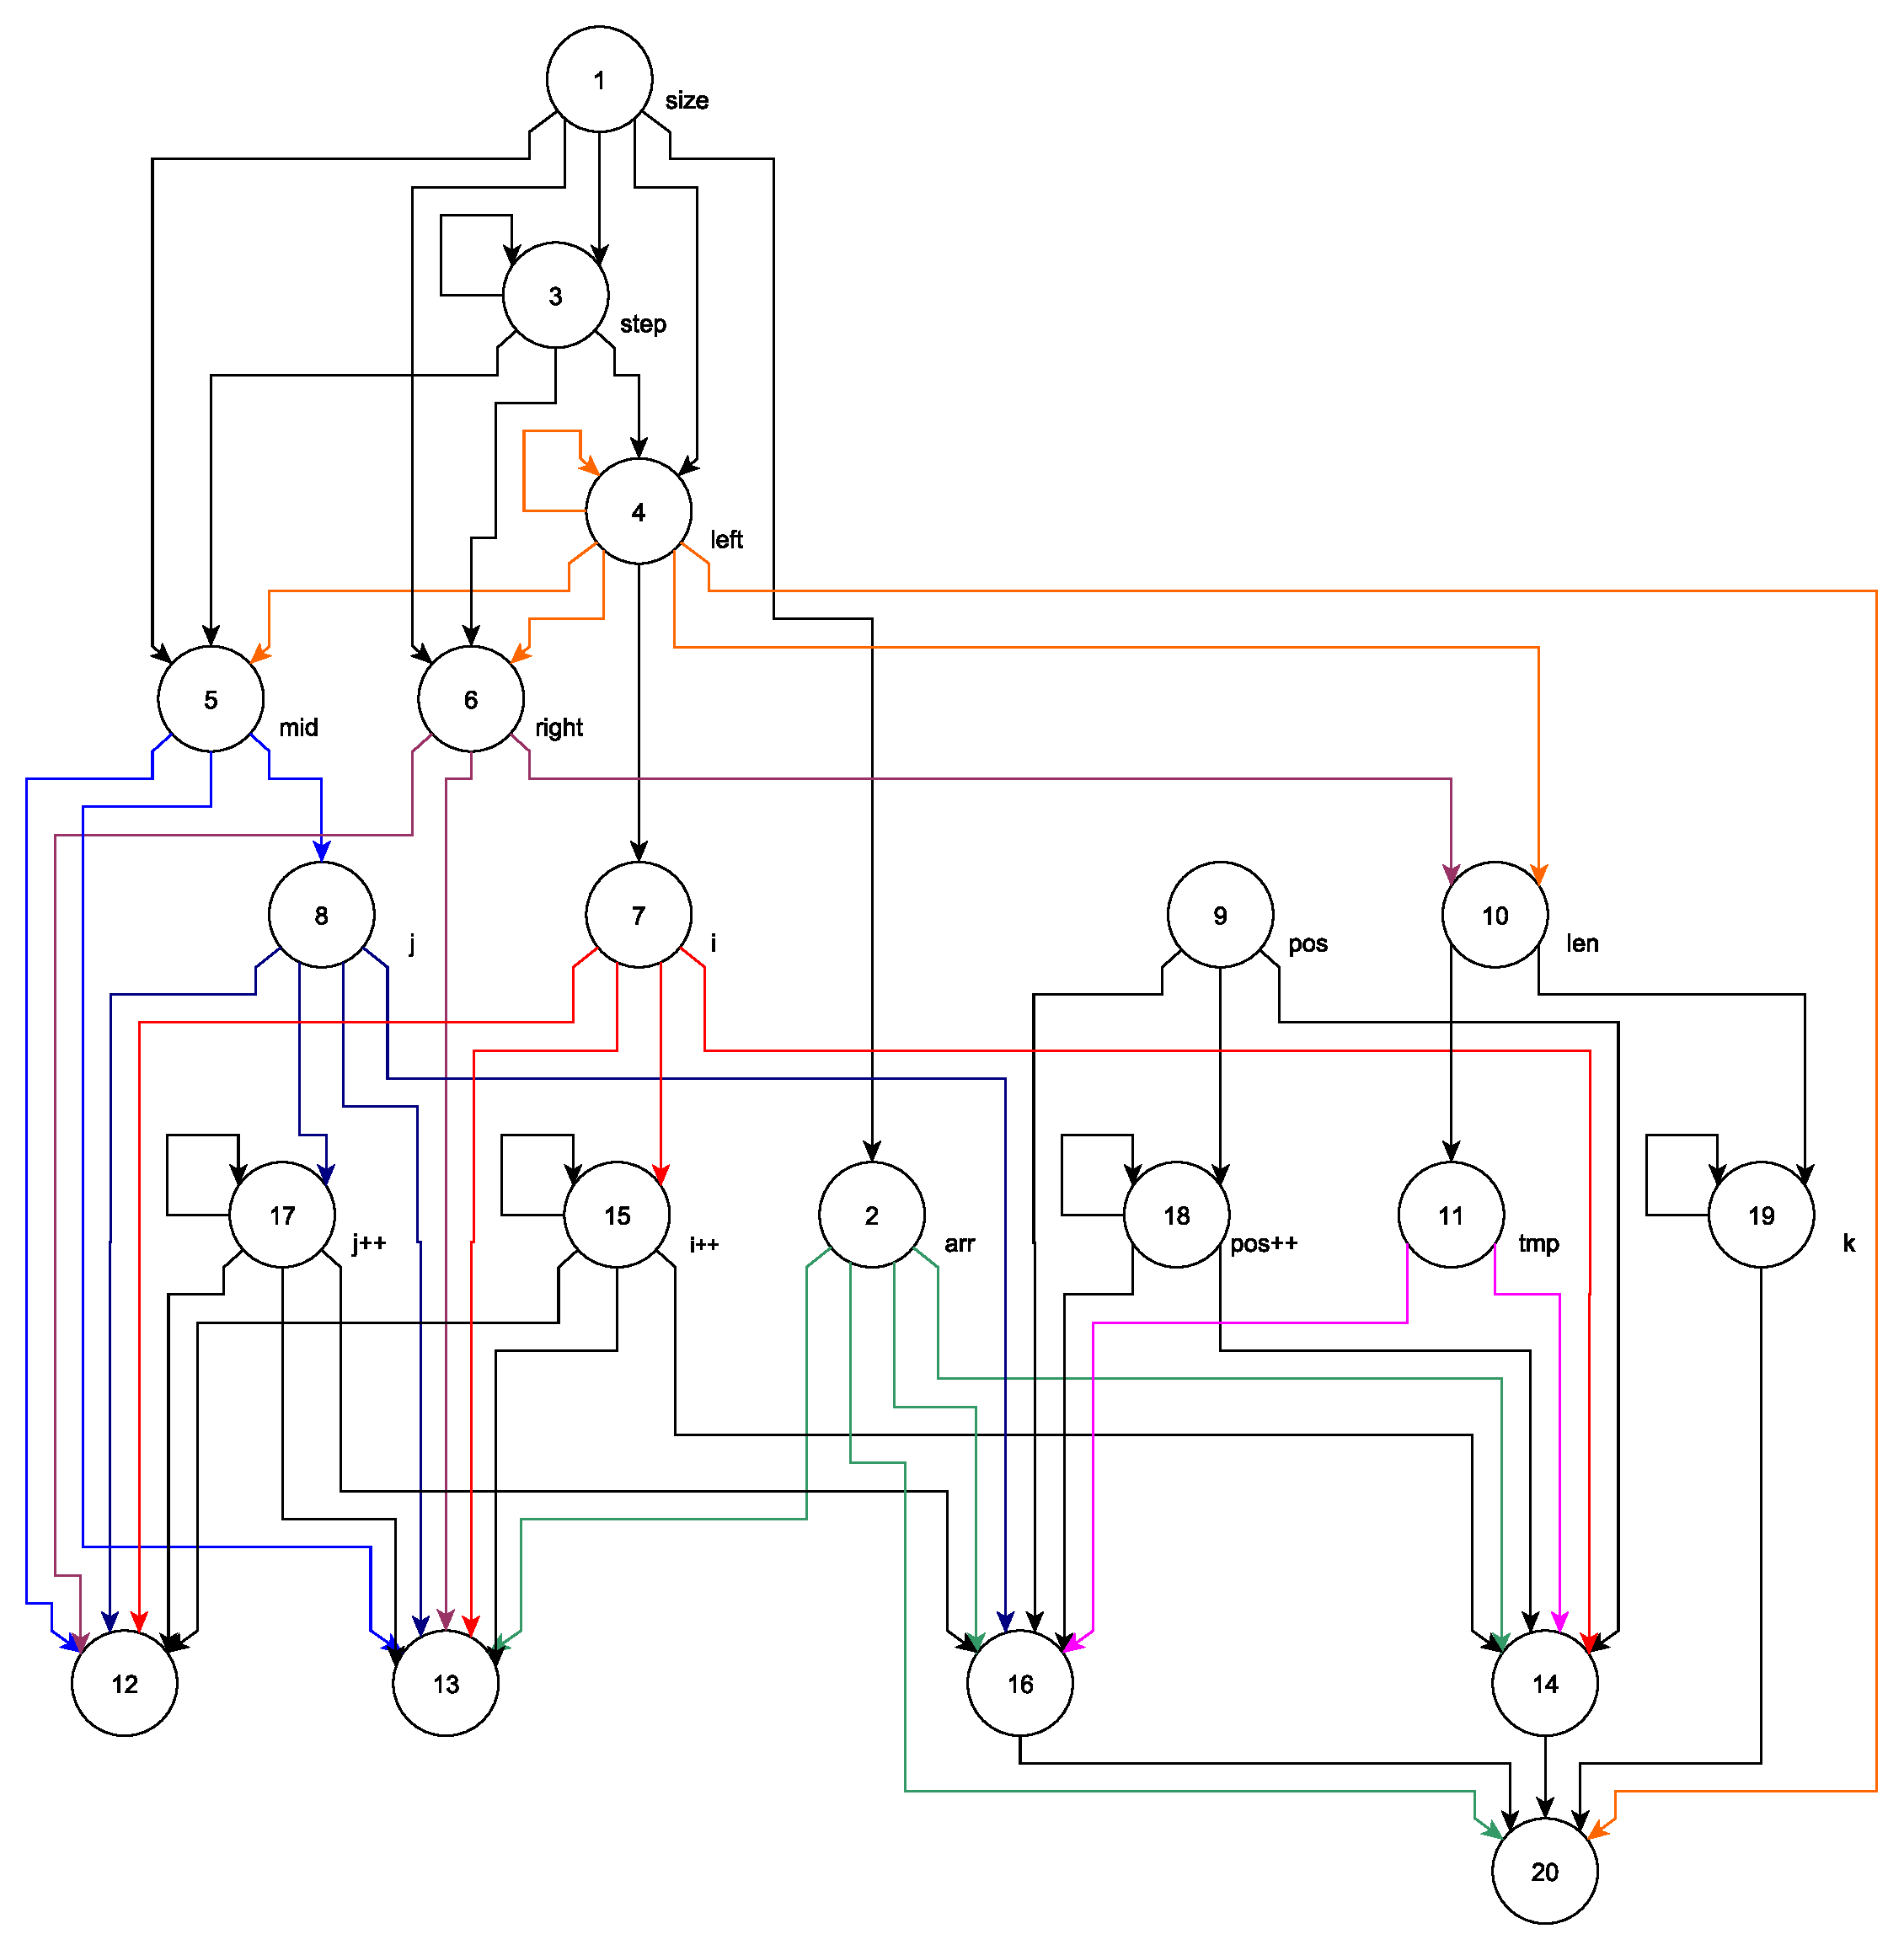
\includegraphics[height=0.5\textheight, page=1]{img/информационный_граф.pdf}
	\caption{Информационный граф}
\end{figure}

\clearpage

\subsection{Операционная история программы}

Рассмотрим следующий массив: \texttt{a = [4, 3, 2, 1]}.

\begin{figure}[h]
	\centering
	\label{fg:os}
	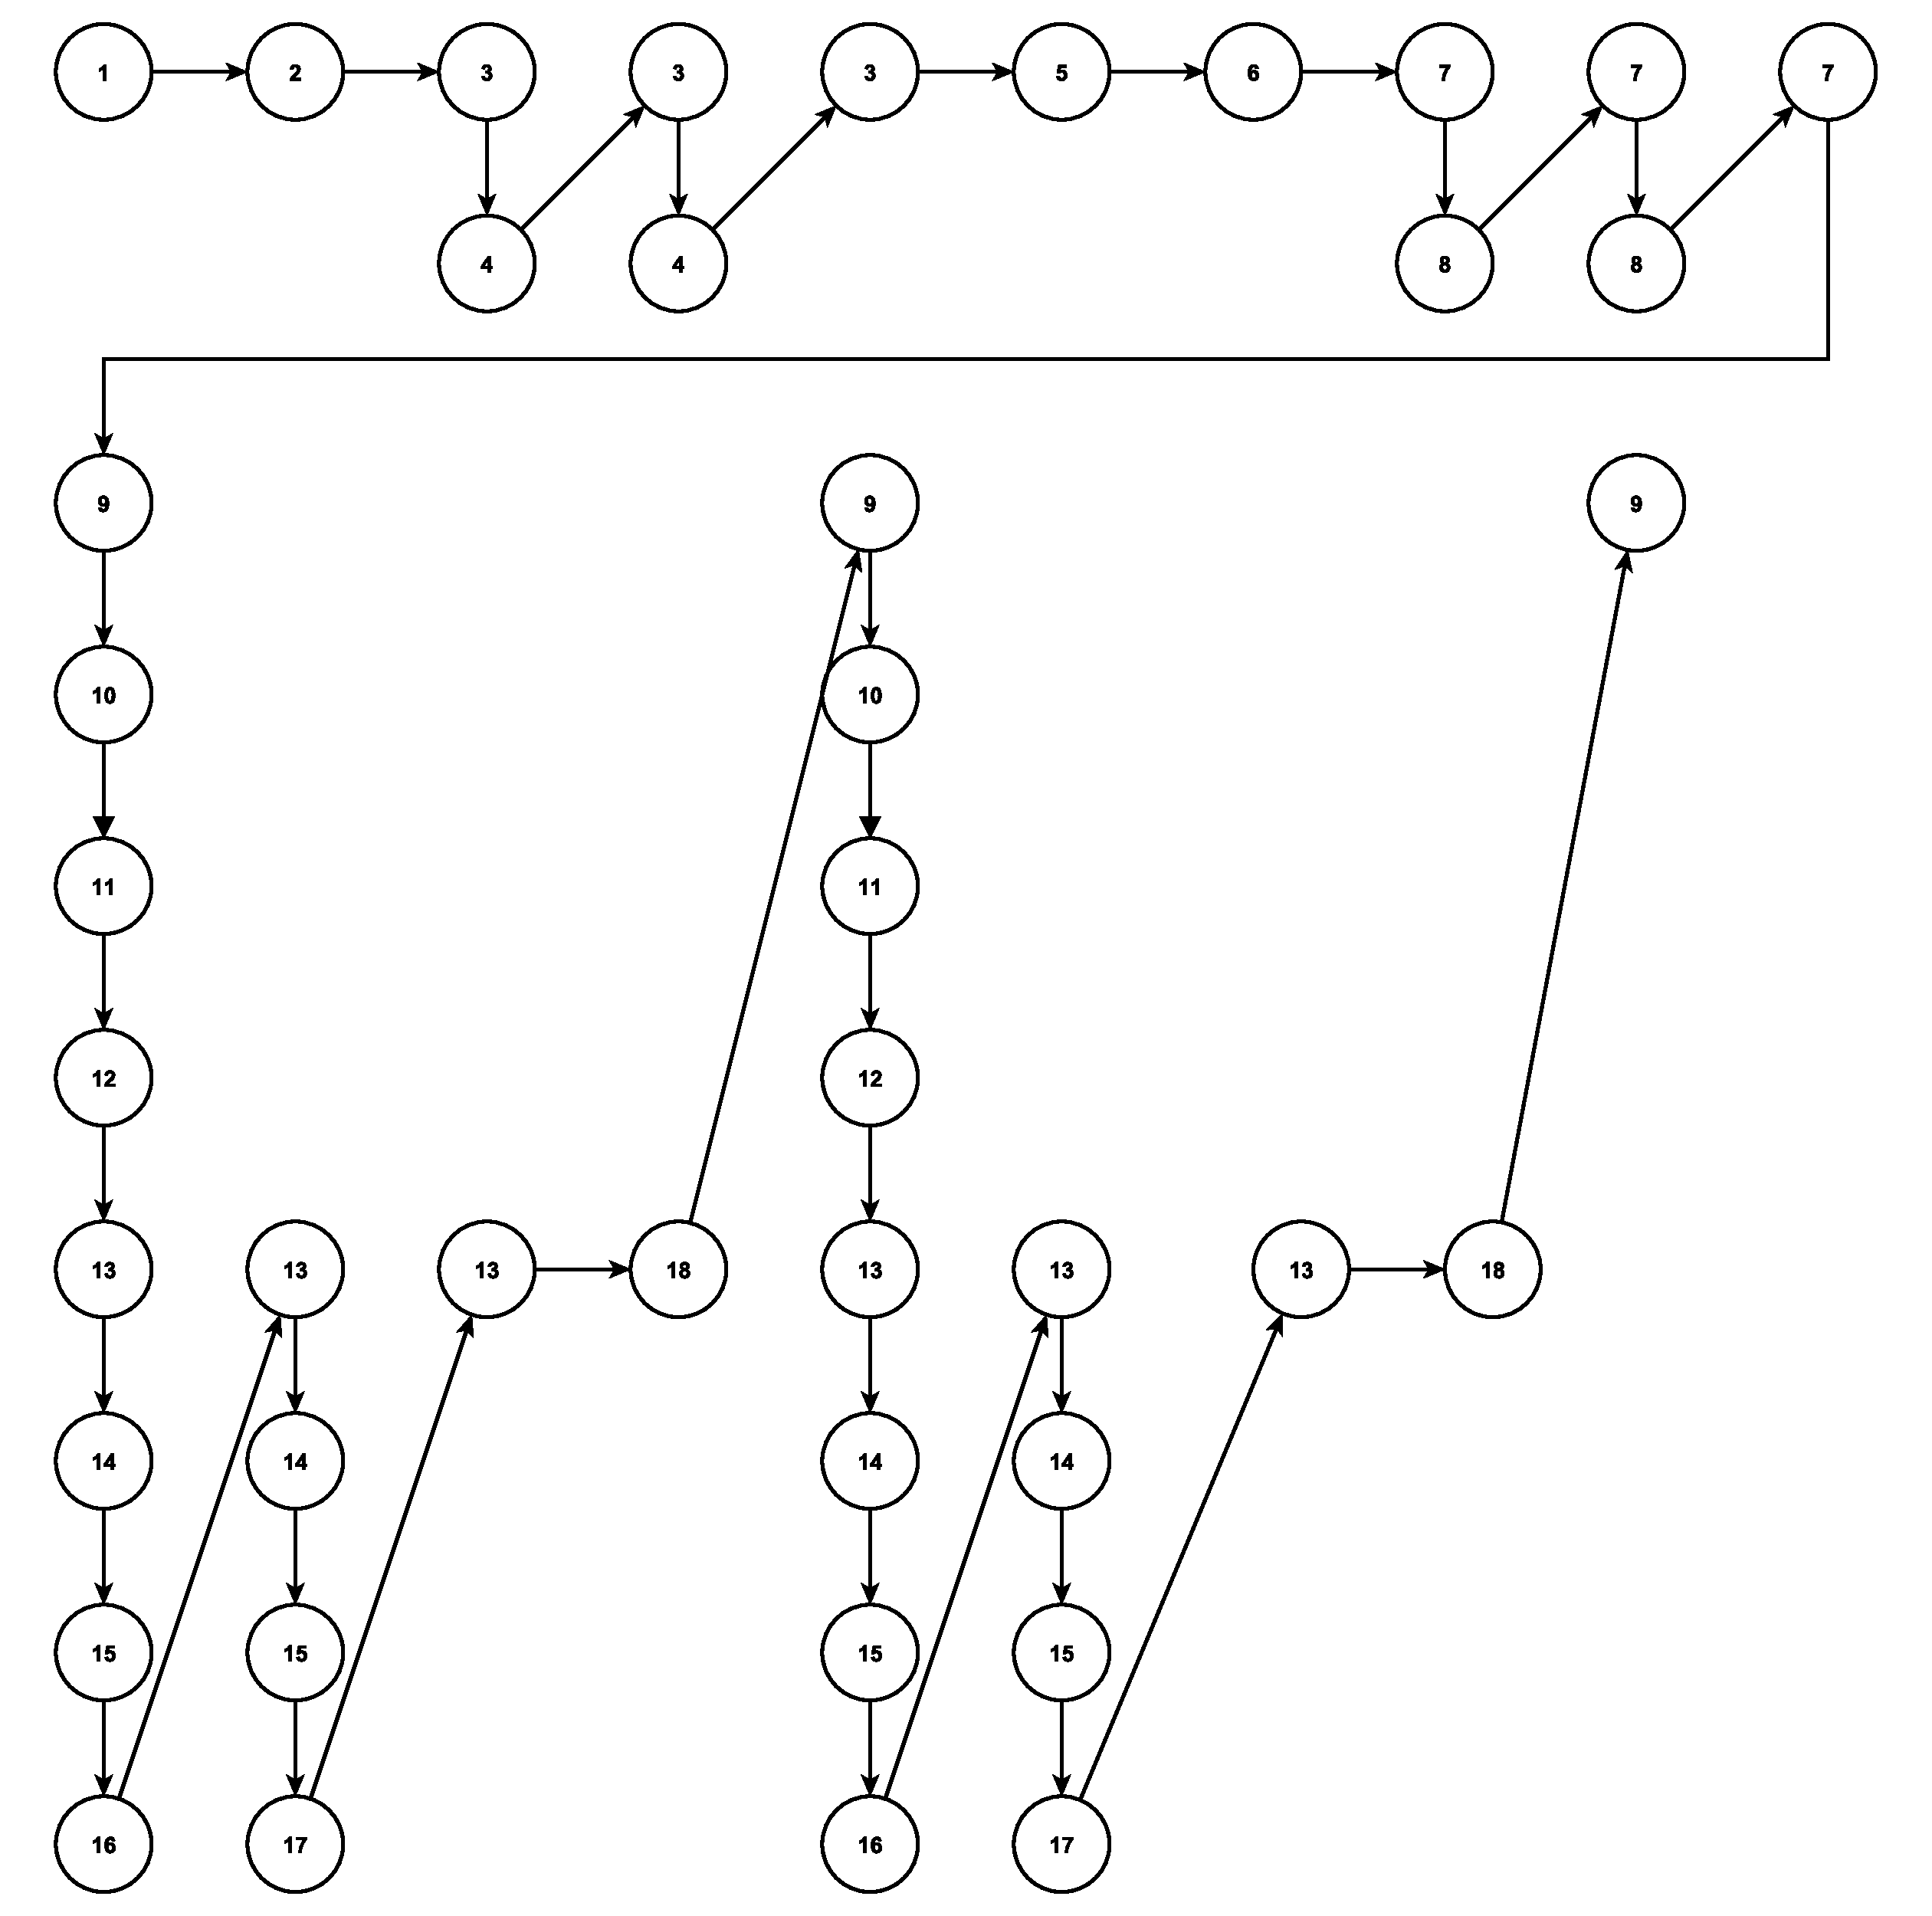
\includegraphics[height=0.7\textheight, page=1]{img/операционная_история.pdf}
	\caption{Операционная история}
\end{figure}

\clearpage

\subsection{Информационная история программы}

\begin{figure}[h]
	\centering
	\label{fg:ii}
	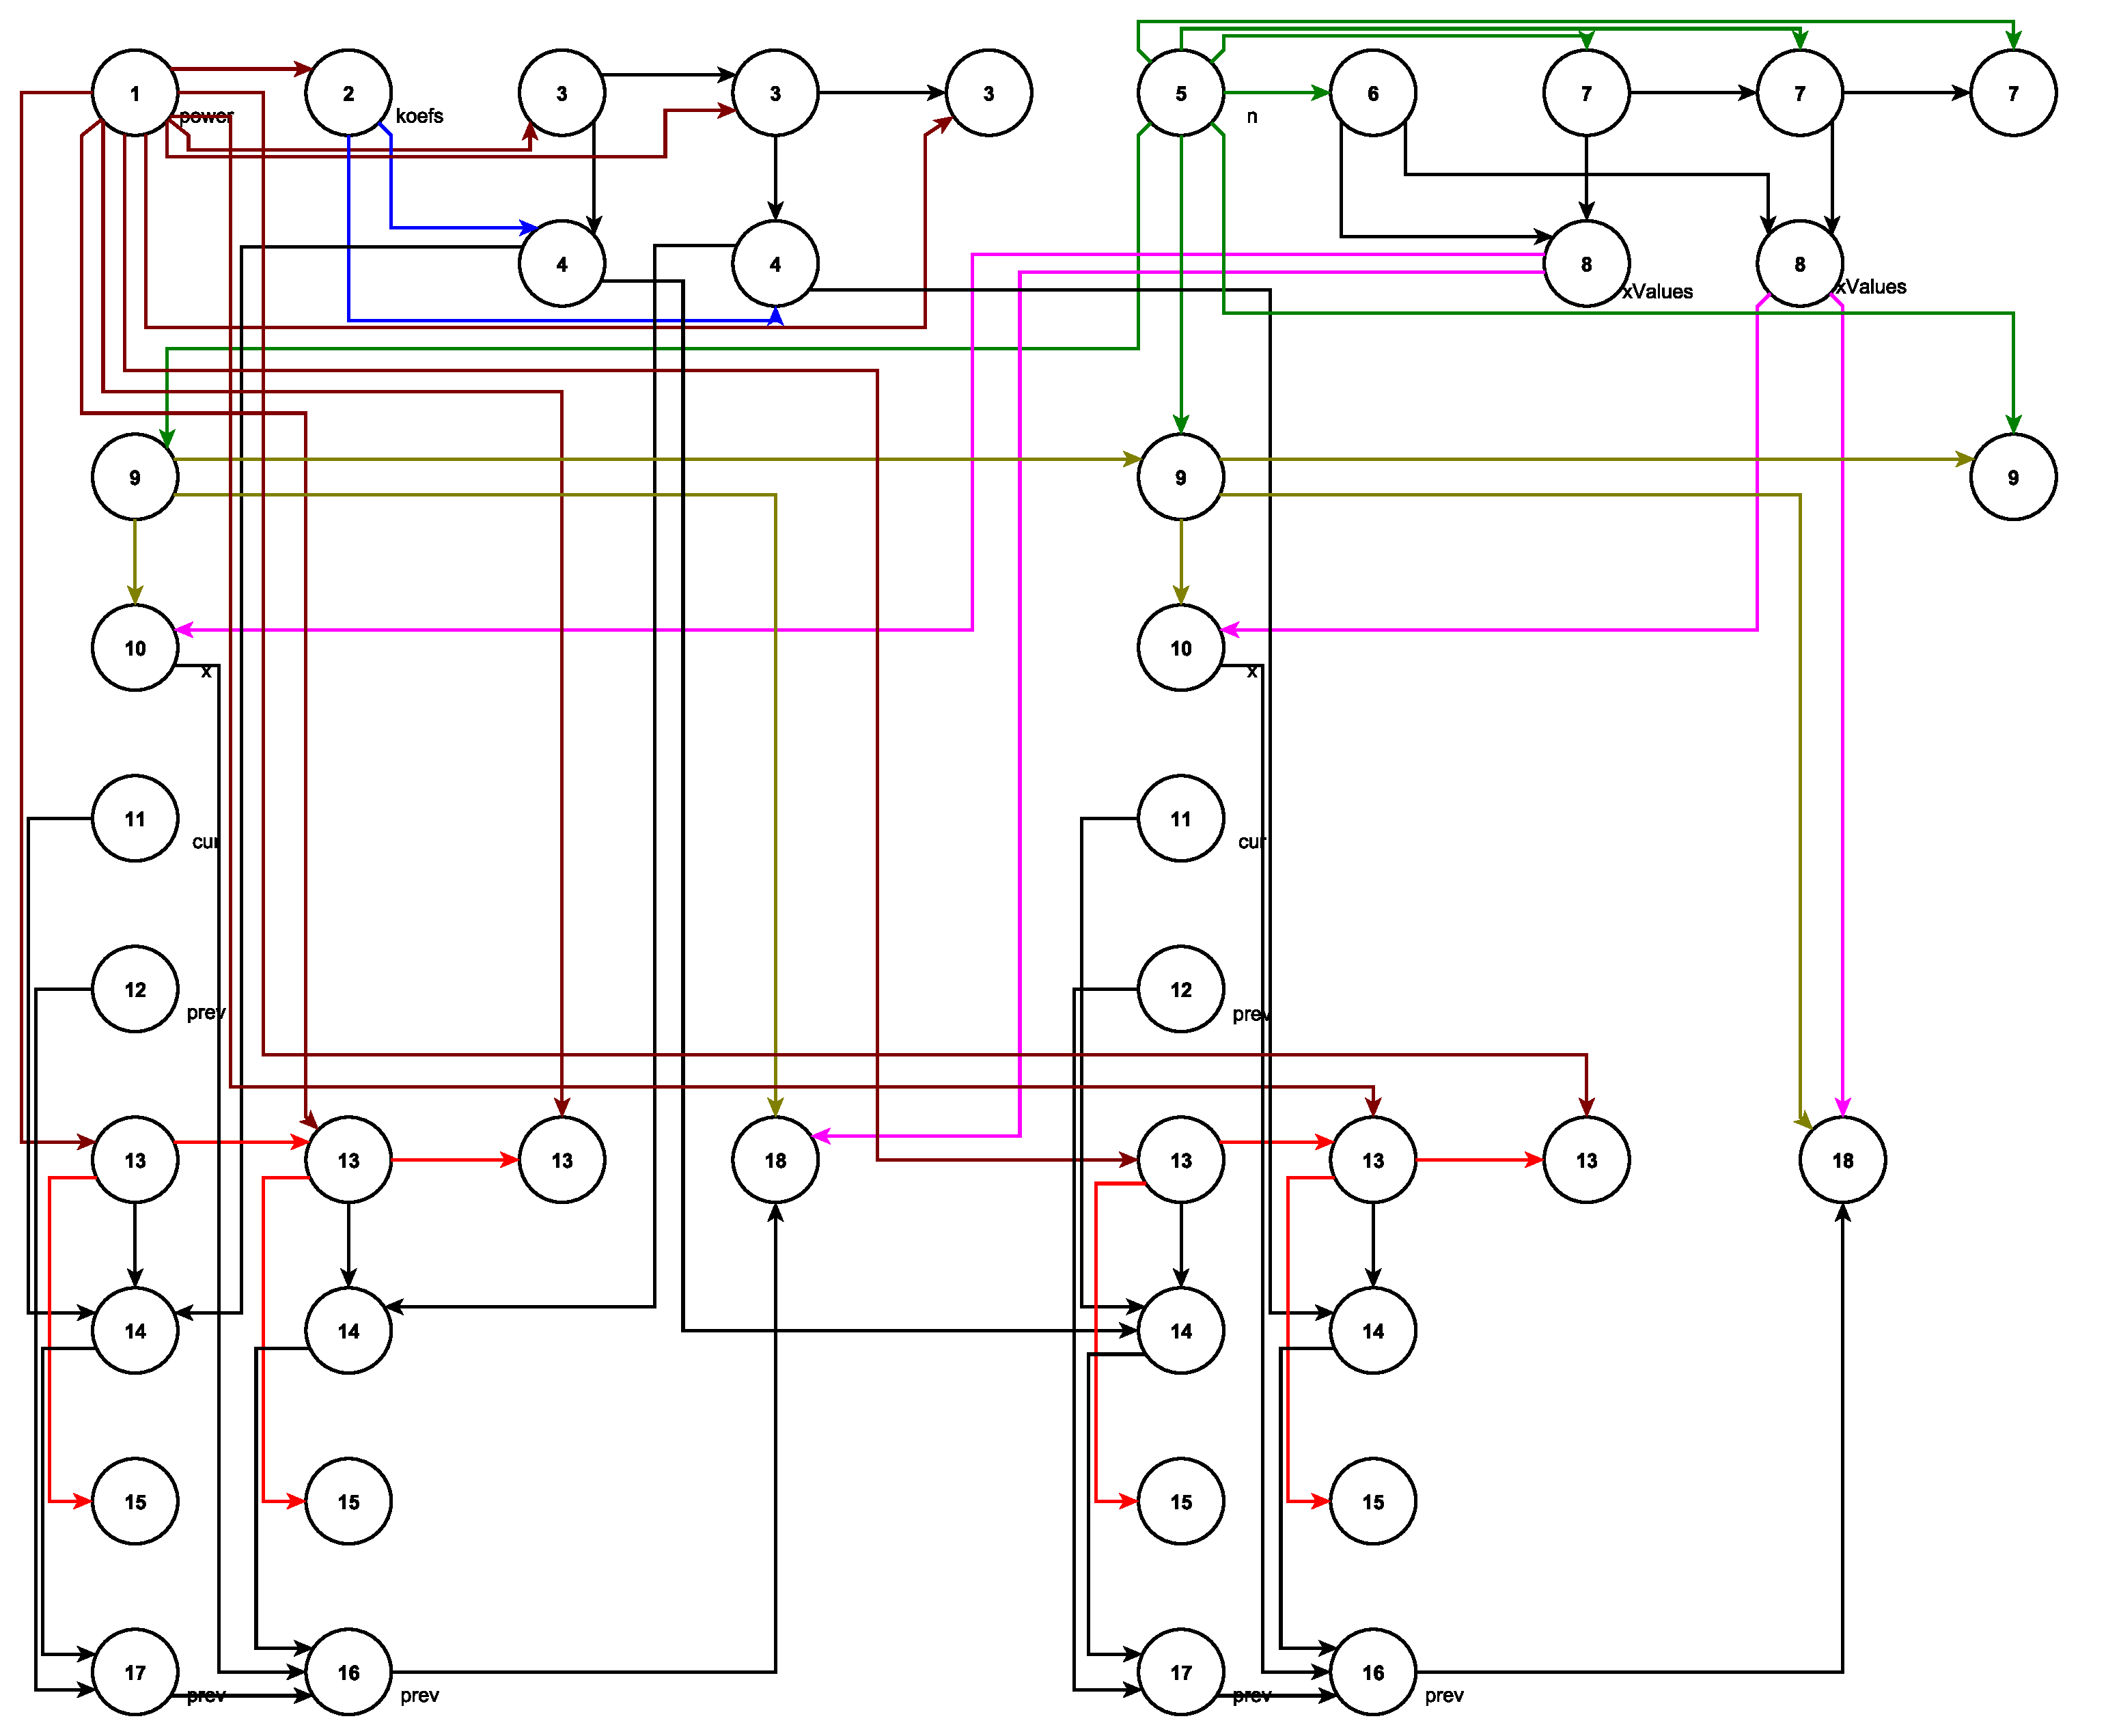
\includegraphics[height=0.7\textheight, page=1]{img/информационная_история.pdf}
	\caption{Информационная история}
\end{figure}

\clearpage

\subsection{Возможность распараллеливания}
Можно разделить массив на части и запустить каждую часть сортировки в отдельном потоке, а затем объединить результаты.